% vim:ts=4:sw=4
%
% Copyright (c) 2008-2009 solvethis
% Copyright (c) 2010-2012 Casper Ti. Vector
% Public domain.

\chapter{Overview}
\section{Experimental Setup}
In our work, a simulator was used to produce the snap assembly process. HIRO, a simulated 6 DoF dual-arm anthropomorph robot was used in the OpenHRP 3.0 environment. CAD derived male and female camera parts were used and the male parts were mounted on the wrist while the female part with 4 snaps was fixed on the ground. The snap part of this task is cantilever snap. The cantilever snap is as the following picture. \\
\begin{figure}
    \centering
    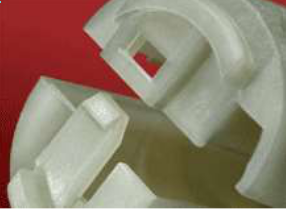
\includegraphics[scale=0.4]{img/cantilever.png}
    \caption{Cantilever Snap}
    \label{snap}
\end{figure}
\indent For controlling, Side Approach strategy is used to assemble the snap parts and Relative Change Based Hirearchical Taxonomy System (RCBHT) is used to sample the force/torque signals of the whole process.
\section{Control Strategy}
The control strategy is fixed. The assembly process contains four state: Approach state, Rotation state, Insertion state, Mating state. In approach state, the upper part approaches to the lower part. After approach state, the upper part rotates until the other two sides of the upper part and the lower part contact. Then force increase to insert the upper part into the lower part. The assembly is finished in Mating state. Details about this can be seen in Appendix.\\
\begin{figure}[h]
    \centering
    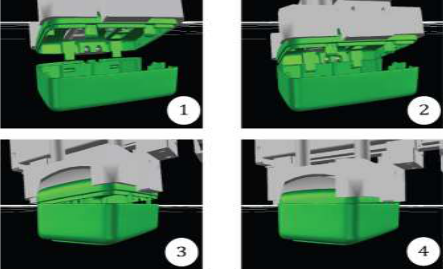
\includegraphics[scale=0.3]{img/controlStrategyFourStep.png}
    \caption{Four control states}
    \label{RCBHT}
\end{figure} 
\section{Relative Change Based Hirearchical Taxonomy System}
The relative change-based hierarchical taxonomy is the state estimation technique that represents the states by hierarchically abstracting snap assembly for force/torque data in increasingly intuitive ways. Five increasingly abstracted layers were used to encode the relative change ub with the force signatures. The taxonomy is consisted by five increasing abstracted layers, including Primitive layer, Motion Composites layer, Low-level Behavior layer, High-level Behavior and Snap Verification Layer. The layers is shown in \\
\begin{figure}[h]
    \centering
    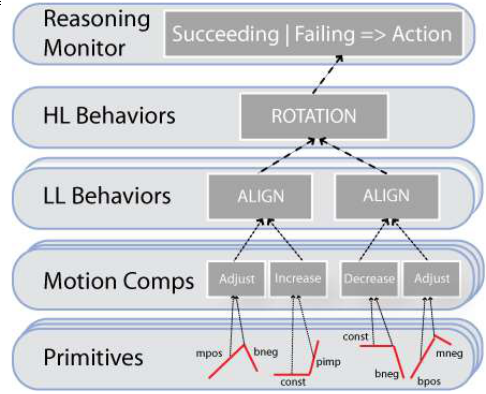
\includegraphics[scale=0.3]{img/fiveLayers.png}
    \caption{Five Layers of RCBHT}
    \label{RCBHT}
\end{figure} 
\indent In our work, we used three lower layers instead the five layers. The details about RCBHT can be seen in \cite{2012IROS-Rojas-RCBHT}. In this section, we will only describe the three lower layers.
\subsection{Primitive layer}
In the primitive layer, each signal is partitioned into linear segments with linear regression with a coefficient. Nine ranges of value of coefficient were labeled by nine different labels. The labels indicate nine ranges of gradients. The upper layers are based on Primitive layer labels.
\subsection{Motion Composites layer}
Motion Composites are consisted of multi-labels of Primitive layer. Two or above similar labels of Primitive layer produced a Motion Composite label. This more abstracted labels attenuate the noise and condense the information.
\subsection{Low-level Behavior leyer}
Being more abstracted, labels of Motion Composite Layer form another layer, Low-level Behavior layer. In this layer, information became more purer and represent the process more intuitively.\\

\indent Details about RCBHT can be seen in appendix.


